\chapter{Problem Description}
Consider a thin film of Silicon with height $H$ and length $L$. All the loadings and geometry are considered to be independent of the third direction, hence the problem is formulated with plane strain assumption. There is an existing solid electrolyte interphase (SEI) layer on top of the Silicon film with a height of $H_{\rm{SEI}}$. The origin is placed at the middle of bottom face of the Silicon film, as shown in figure \ref{fig:probDesc}. The bottom face of the Si thin film is considered to be rigidly fixed to a metallic substrate. The left and right faces are considered to have a roller type boundary condition for both Si and SEI. A uniform flux of Li-ions from the top surface of SEI is present. 
\begin{figure}[H]
    \centering
    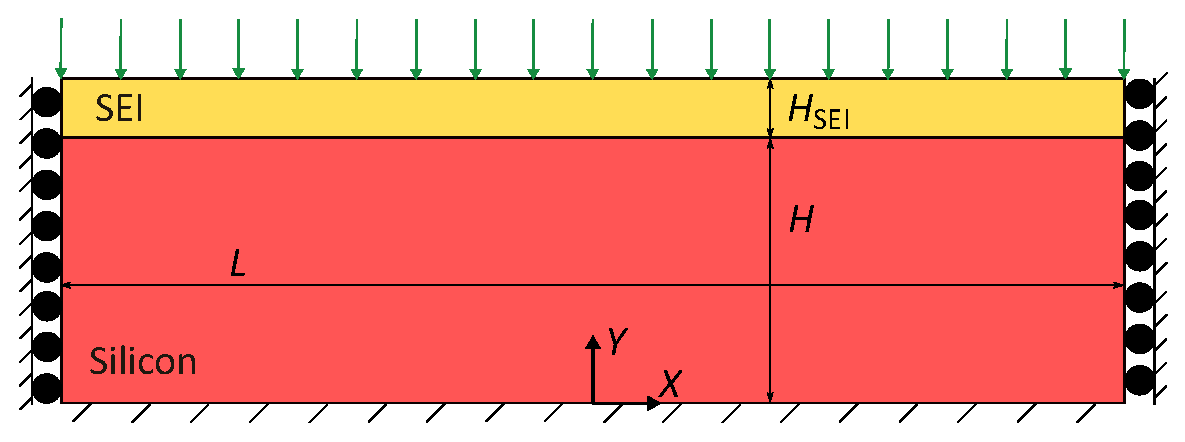
\includegraphics[width=\textwidth]{figures/probDescFigs/drawing.eps}
    \caption{Schematic of the problem showing geometric parameters and boundary conditions.}
    \label{fig:probDesc}
\end{figure}
SEI is considered to be completely permeable to Li-ions and thus doesn't undergo any deformation due to lithiation. In the Silicon thin film, the diffusion leads to a stress field. This is termed as diffusion induced stress (DIS) in the literature. The stress field in turn affects the process of diffusion called stress enhanced diffusion (SED). This leads to two way coupled system of PDEs.
Due to large deformation of the Si during lithiation, it is necessary to formulate the problem with finite deformation theory with an elasto-plastic constitutive behaviour. In the present study, both Si and SEI are considered to exhibit a viscoplastic nature. The constitutive law for elastic regime is taken to be isotropic and concentration dependent for Silicon film and constant for SEI. 
For Mechanical equilibrium, a quasi-static model is employed.